\section{Memory Models}

\lstinline{volatile} garantiert immer Visiblity/Ordering und Atomarität innerhalb einer Operation auch bei Datentypen grösser als 32 Bit \textcolor{red}{nicht aber ++/--/-=/...}

\subsection{Atomicity}
Primitive Datentypen (32 Bit) int, bool, char, short, byte, Objekt-Referenzen, long/double mit \lstinline{volatile} atomar


\textbf{Atomare Operation - Java}

\textcolor{red}{Starvation-Problem!}

\begin{lstlisting}
private final AtomicReference<Node> top = new AtomicReference<>();
boolean success;
do {
    Node current = top.get(); // lese aktuellen Wert
    Node node = new Node(value, current); // Changes or checks (if)
    success = top.compareAndSet(current, node); // schreibe, falls gelesener Wert immer noch aktuell ist
} while (!success); // ev. Thread.yield(); nutzen um temp. 'Focus' abzugeben
.
\end{lstlisting}

\begin{lstlisting}
public class SpinLock {
  private AtomicBoolean locked = new AtomicBoolean(false); // Initialwert false
  public void acquire() {
    while (locked.getAndSet(true)) { } // Lese alten Wert und setze neuen Wert atomar (Rückgabe = gelesener Wert)
  public void release() {
    locked.set(false); } } // Setze false und mache sichtbar
\end{lstlisting}

\lstinline{boolean compareAndSet (boolean expect, boolean update)} Setzt update, wenn Wert gleich expect ist (atomar), retourniert true bei erfolgreichem Update \lstinline{addAndGet()} \lstinline{getAndAdd()}

\begin{lstlisting}
AtomicInteger squares = new AtomicInteger(0);
squares.updateAndGet(x -> x * x); // mit Lambda
\end{lstlisting}

lock-freie BankAccount Klasse

\begin{lstlisting}
public class BankAccount {
  private AtomicInteger balance = new AtomicInteger(0);
  public void deposit(int amount) { balance.getAndAdd(amount); }
  public boolean withdraw(int amount) {
    int oldValue;
    do {
      oldValue = balance.get();
      if(oldValue < amount){ return false; }
    } while (!balance.compareAndSet(oldValue, oldValue - amount));
    return true;
  }
  public int getBalance() { return balance.get(); } }
\end{lstlisting}

%\textbf{lock-freie BankAccount Klasse - .NET}
%
%\begin{lstlisting}
%public class BankAccount {
%  private int balance = 0;
%  public int Balance {
%    get { return Thread.VolatileRead(ref balance); }
%    private set { balance = value; } }
%
%  public void Deposit(int amount) { Interlocked.Add(ref balance, amount); }
%  public bool Withdraw(int amount) {
%    int oldValue;
%    do {
%      oldValue = Balance;
%      if (oldValue < amount) { return false; }
%    } while (oldValue != Interlocked.CompareExchange(ref balance, oldValue - amount, oldValue));
%    return true; } }
%\end{lstlisting}

\subsection{Visibility}

Thread bekommt Variablenänderung/-manipulation eines anderen Threads nicht mit (Änderung wird nicht sichtbar) $\rightarrow$ Endlos-Loop weil gleicher Wert \textcolor{red}{gitb es bei .Net nicht!}

\textcolor{blue}{Lock-Release \& -Acquire} Änderungen vor release werden bei acquire sichtbar

\textcolor{blue}{Volatile Variable} möchten alles vorherige sehen

\subsection{Ordering}

\textcolor{blue}{Program Order (as-if-serial)} Sequenzielles Verhalten jedes einzelnen Threads bleibt erhalten

\textcolor{blue}{Synchronisation Order (Total Order)} Synchronisationsbefehle werden zueinander nie umgenordnet (Locking, volatile, Thread Start/Join)

\textcolor{blue}{Happens-Before Relation (Partial Order)} \textcolor{red}{Alles andere kann umgeordnet werden!}

\textbf{.NET Ordering} \textcolor{red}{volatile schützt nicht vor Ordering!}

\begin{minipage}[t]{0.3\linewidth}
    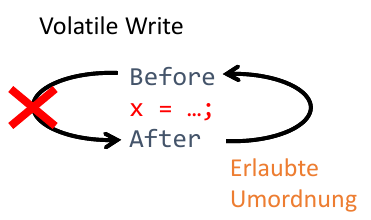
\includegraphics[width=\linewidth]{03_net-ordering-1.png}
\end{minipage}
\begin{minipage}[t]{0.3\linewidth}
    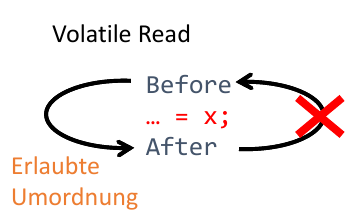
\includegraphics[width=\linewidth]{03_net-ordering-2.png}
\end{minipage}
\begin{minipage}[t]{0.3\linewidth}
    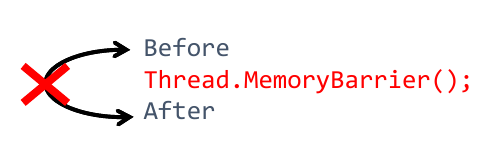
\includegraphics[width=1.2\linewidth]{03_net-ordering-barrier.png}
\end{minipage}

